\section{Hardware dell'adapter board}
L'hardware utilizzato per condurre lo studio oggetto di questa tesi consiste in due piattaforme indossabili per effettuare misure fotopletismografiche. Ciascuna piattaforma si compone di una Adapter Board e una scheda ospitante un microcontrollore. L'Adapter Board consiste in una PCB sulla quale sono montati il modulo PPG, un accelerometro ed un eventuale LDO per l'alimentazione dei componenti. Il microcontrollore viene utilizzato per l'acquisizione dei dati dai sensori e per il loro controllo. In particolare è stata utilizzata in entrame le soluzioni la board \textbf{STM32F4DISCOVERY}, prodotta da STMicroelectronics che ospita il microntrollore \textbf{STM32F407}.
La due piattaforme progettate si differenziano per l'Adapter Board, dal momento che sono stati utilizzati due differenti moduli PPG: il \textbf{MAXM86161} e il \textbf{MAX86916}. Entrambi i sensori sono prodotti da Maxim Integrated.
\subsection{Adapter Board: MAXM86161}
\begin{figure}[b]
	\centering
	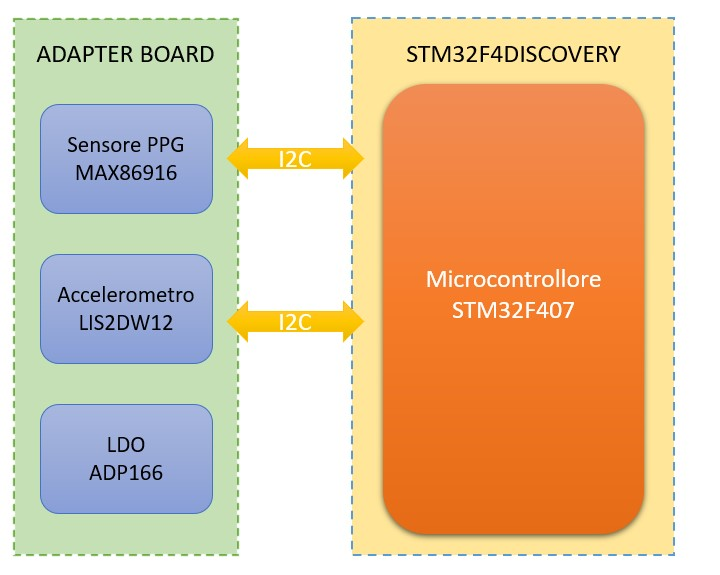
\includegraphics[width=0.6\linewidth]{ImageFiles/Hardware/DiagrammaBlocchiMAXM86161}
	\caption{to be done}
	\label{fig:DiagrammaBlocchiMAXM86161}
\end{figure}
\todo{aggiungerei all'immagine anche la usb come avevamo detto in modo che si veda poi come comunicheremo con il pc. ocio ai componenti... verificare sempre su eagle}
L'Adapter Board progettata ospita il sensore PPG MAXM96161 e l'accelerometro triassiale LIS2DW12, che comunicano con il microcontrollore tramite protocollo I\ap{2}C (\Fig~\ref{fig:DiagrammaBlocchiMAXM86161}). Grazie al numero ridotto di componenti è stato possibile ottenere una scheda dalle dimensioni molto ridotte (12,4 mm x 4,6 mm).

\paragraph{Sensore PPG} Il sensore PPG utilizzato è il MAXM86161 rappresentato nella figura \ref{fig:ImmagineMAXM86161}.
\begin{figure}[tb]
	\centering
	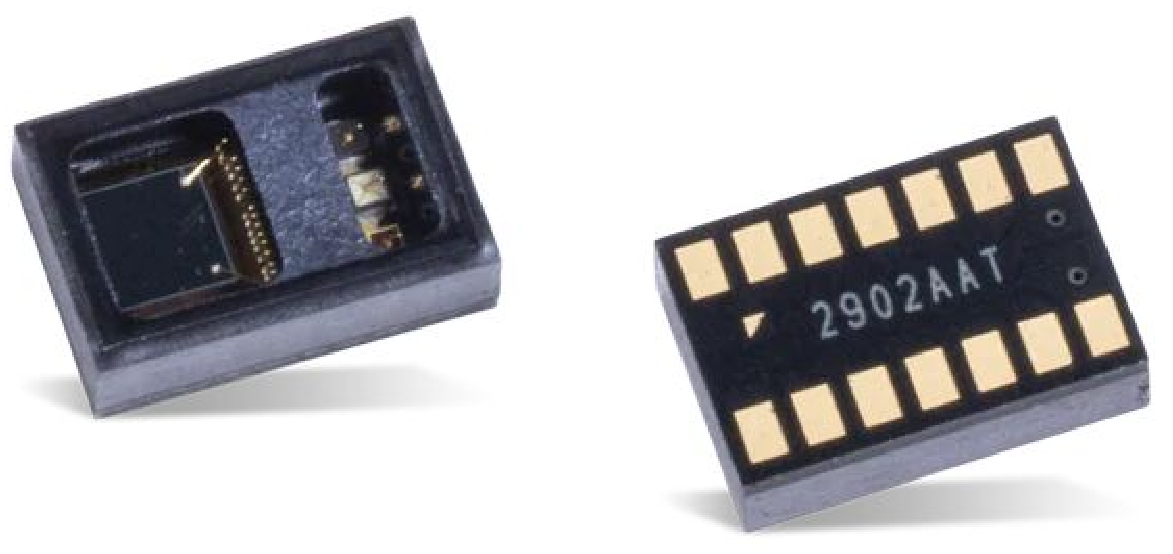
\includegraphics[width=0.8\linewidth]{ImageFiles/Hardware/ImmagineMAXM86161}
	\caption{MAXM86161 magari evidenziare i led e fotodiodo}
	\label{fig:ImmagineMAXM86161}
\end{figure}
Si tratta di un modulo integrato a basso consumo, per acquisizioni di dati ottici. Il sensore integra 3 LED (rosso, infrarosse e verde), un fotodiodo e un regolatore di tensione lineare (LDO). Per questo motivo non è necessario inserire un ulteriore LDO esterno per l'alimentazione dei circuiti interni e dei LED. \`E presente un pin di uscita (VLDO) collegato all'uscita del regolatore interno che fornisce una tensione di 1.8V. Essa può essere utilizzata per alimentare eventuali dispositivi esterni. Il MAXM86161 necessita di una singola tensione di alimentazione che deve essere compresa tra i 3.0V e 5.5V. Presenta un package di tipo OLGA a 14 pin, con dimensioni 2.9 mm x 4.3 mm x 1.4 mm. La comunicazione con il microcontrollore avviene grazie alla presenza dei pin SDA e SCL, tipici della comunicazione I\ap{2}C.\todo{inserire riferimenti al pin di interrupt}

\paragraph{Accelerometro}\todo{da rivedere}

\cite{STElectronicsLIS2DW12}

% Insieme alle acquisizioni del sensore PPG vengono integrate anche delle misure accelero-metriche. L'accelerometro utilizzato è \textbf{LIS2DH12} \cite{STMicroelectronicsLIS2DH12} prodotto da STMicroelectronics. Si tratta di un accelerometro triassiale a basso consumo e dalle piccole dimensioni (2 x 2 mm). Questo sensore viene utilizzato per migliorare la qualità delle acquisizioni fotopletismografiche quando il soggetto è in movimento, fornendo un'informazione sull'entità di quest'ultimo, e quindi del disturbo che si introduce nella misura. Il LIS2DH12 richiede una tensione di alimentazione compresa tra i 1.71V e i 3.6V, con un consumo di corrente pari a \SI{185}{\micro\ampere}.
\todo{inserirei come in facagni la tabella dei componenti}
\paragraph{Progetto PCB}

\subsection{Adapter Board: MAX86916}

\paragraph{Sensore PPG} Il sensore PPG utilizzato è il MAX86916, prodotto da Maxim Integrated, descritto precedentemente come stato dell'arte.

\begin{figure}[tb]
	\centering
	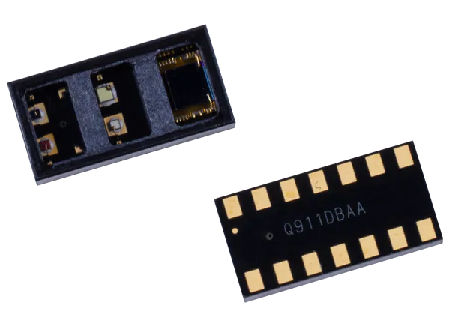
\includegraphics[width=0.6\linewidth]{ImageFiles/Hardware/ImmagineMAX86916}
	\caption{MAX86916 magari mettere in evidenza led e foto diodo}
	\label{fig:ImmagineMAX86916}
\end{figure}

\paragraph{LDO} \todo{Parliamo dei 3 LDO che abbiamo valutato? si parlerei di tutti e tre o almeno 2 mettendo in evidenza magari una tabella con le differenze}

\paragraph{Accelerometro}\todo{ut supra} L'accelerometro utilizzato è sempre \textbf{LIS2DH12} prodotto da STMicroelectronics.

\subsection{Microcontrollore: STM32F4DISCOVERY}\todo{farei una descrizione con alcune nozione sui componenti}
\todo{inserire immagine della board}